\noindent

Dans cette partie nous décrivons les grands types de données sur lesquelles repose le calcul du problème direct par OpenMEEG.
Pour des détails sur les structures de données, on se reportera à l'Annexe~\ref{chap:formats}.

\noindent
\underline{Maillages}~:\\
il faut définir des maillages pour les interfaces des différents domaines de conductivité. Il s'agit, généralement de trois maillages~: 
\begin{itemize}
    \item un maillage grossier de la surface extérieure du cortex,
    \item un maillage de la surface extérieure du crâne,
    \item un maillage pour la surface extérieure scalp. 
\end{itemize}

\noindent
La taille recommandée pour ces maillages est d'environ  600 à 800 points par surface. 

\medskip

\centerline{
    \hbox{\parbox[t]{5.5cm}{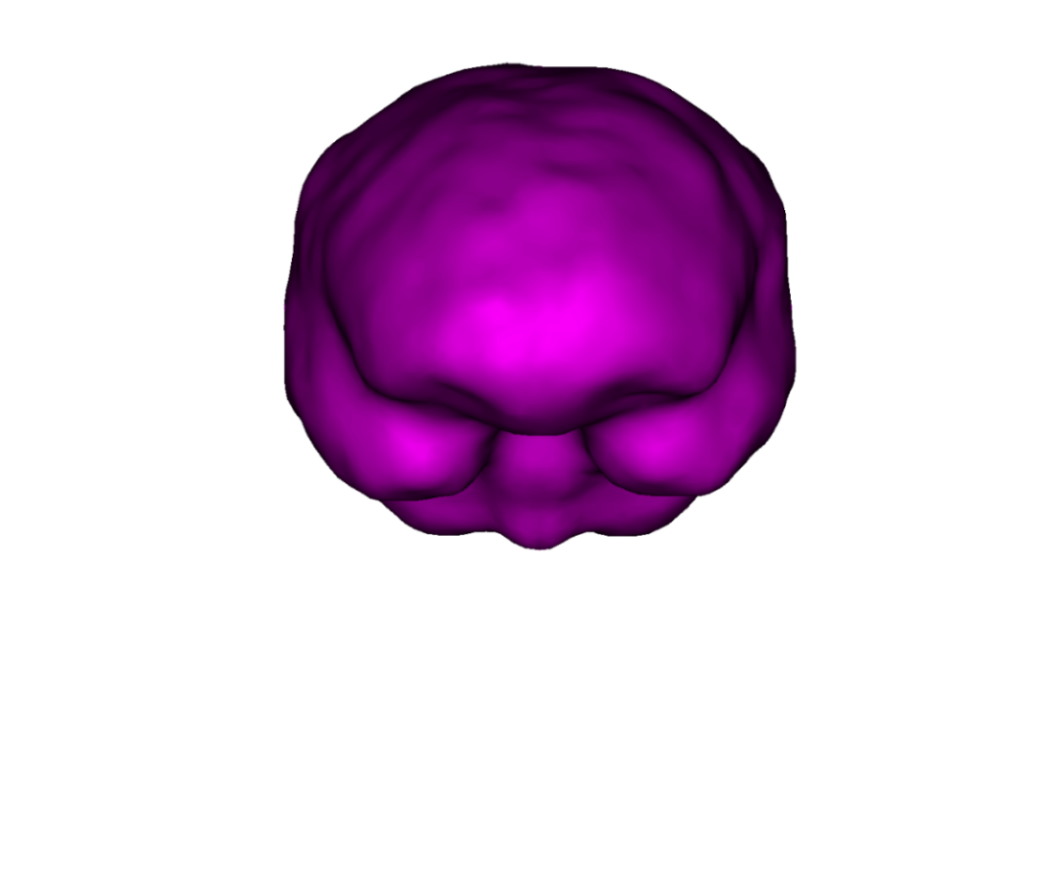
\includegraphics[width=5cm]{tete_couches_brain.png}\\
                            \parbox{5cm}{Surface extérieure au cortex}}
          \parbox[t]{5.5cm}{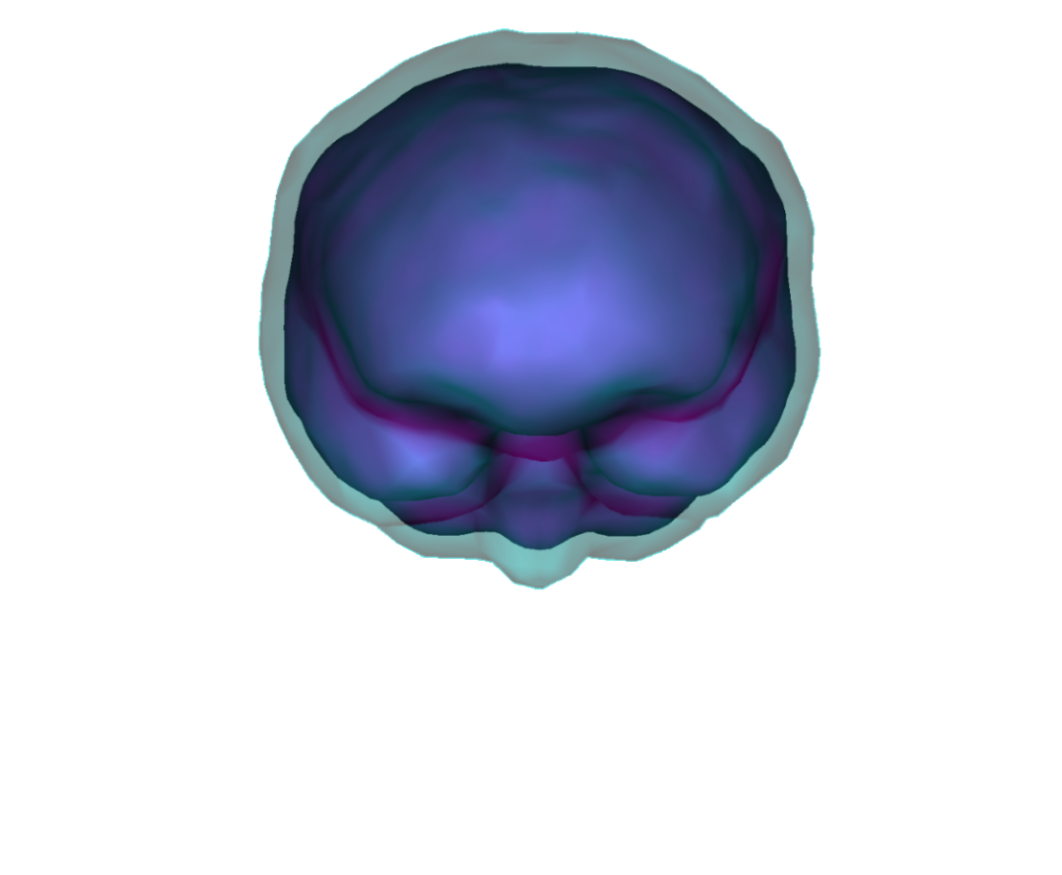
\includegraphics[width=5cm]{tete_couches_brainskull.png}\\\parbox{5cm}{Surface extérieure au crâne en bleu et surface extérieure au cortex en fushia}}
          \parbox[t]{5.5cm}{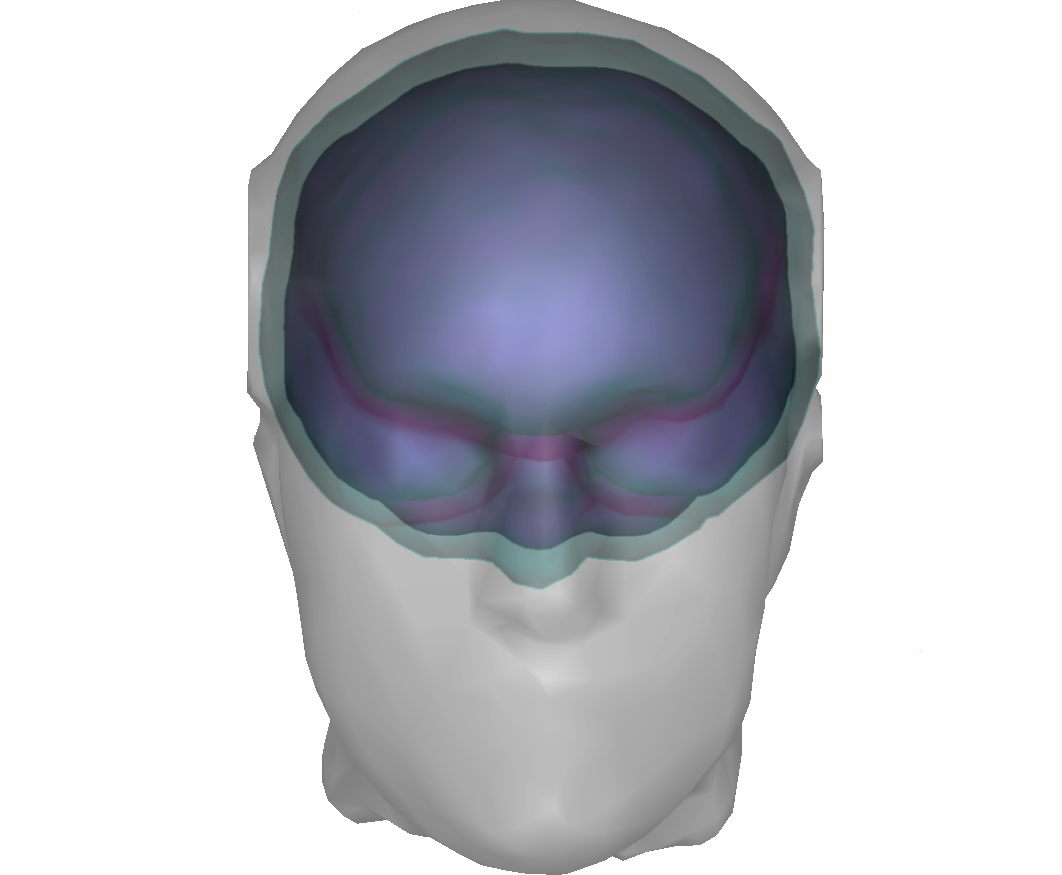
\includegraphics[width=5cm]{tete_couches_brainskullhead.png}\\
                            \parbox{5cm}{Exemple avec trois surfaces~:
                                  \begin{itemize}
                                       \item extérieure au scalp en gris
                                       \item extérieure au crâne en bleu
                                       \item extérieur au cortex en fushia
                                  \end{itemize}}
                            }
    }
}

\bigskip

\noindent
\underline{Sources}~:\\
Les sources peuvent être de deux types: isolées ou distribuées.
\noindent
Dans le cas de sources distribuées, il faut un maillage représentant le support des sources. Il s'agit généralement d'un maillage détaillé du cerveau, dont la taille peut varier de 10 000 et 30 000 points.
Les sources représentées par un maillage ont une amplitude  {\em continue} et linéaire sur chaque triangle de la surface maillée. Cette amplitude est discrétisée par des éléments finis P1 (polynomiaux de degré un).
L'orientation des sources est constante par morceaux, d'orientation normale à chaque triangle.
\begin{center}
    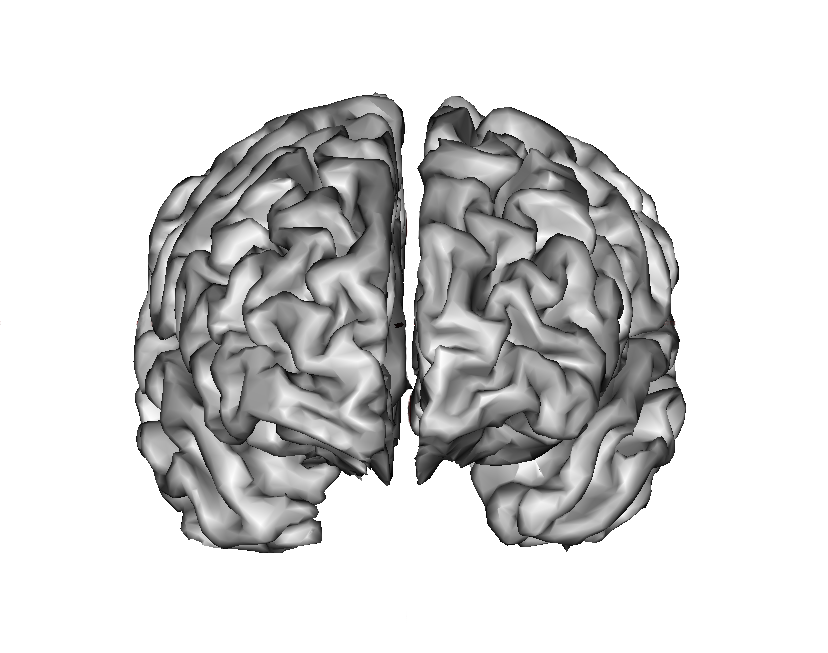
\includegraphics[height=9cm]{cortex.png}\\
    Maillage de sources
\end{center}
\noindent
Des sources isolées sont constituées d'une superposition de dipoles de courants ponctuels, chacun défini par sa position et son moment. 

\noindent
\underline{Capteurs}~:
	Dans le cas de l'EEG, un fichier de description de la position des électrodes (ou patches) en coordonnées cartésiennes.
Dans le cas de la MEG, les capteurs sont plus complexes à décrire, cf l'Annexe~\ref{sec:sensors}.
